 \subsection{Statistics}

 We call \textit{statistic} an   index related to a rv. Examples are the mean, the (co)variance, the standard deviation, the correlation ...

 We first introduce the \textit{expected value}, a central concept in ML, of a function $g(x)$ of a univariate discrete rv X with probability density function $p(x)$ as:
   $$\mathbb{E}_X[g(x)]=\sum_{x \in S_X} g(x)p(x)dx$$
   where $S_X$ is the target space of the rv X.
  
   If we consider a multivariate random variables $X=(X_1, \ldots X_D)$ the expected value is a vector containing as elements the expected values with respect to the single rv $X_i, i=1, \ldots D$.
   $$ \mathbb{E}_X[g(\xx)]=\begin{matrix} 
   \mathbb{E}_{X_1}[g(x_1)] \\
   \ldots \\
   \mathbb{E}_{X_D}[g(x_1)] 
   \end{matrix}
   $$
  

   \begin{definition} 
   The \textit{mean} of a univariate rv X with states $(x_1, \ldots x_m)$ is an average defined as:   $$\mathbb{E}_X[\xx]=\sum_{x_i \in S_X}x_i p(x_d=x_i)$$
   \end{definition}
   
The extension to the multivariate rv $X=(X_1, \ldots X_D)$ is made as before.
   
For univariate rv $X$ we can also define the median as a measure of the center of the distribution.
 For two univariate rv $X$ and $Y$ we can define the covariance statistic which measures \textit{how independent} the two variables are. 
  
  
   Let $\mu_X=\mathbb{E}_X[\xx]$ and $\mu_Y=\mathbb{E}_Y[\yy]$.
 \begin{definition}
     We define the \textit{covariance} between two random variables $X$ and $Y$ as
     $$ \text{Cov}[x, y] = \mathbb{E}[(x - \mu_X)(y - \mu_Y)] = \mathbb{E}[xy] - \mathbb{E}[x]\mathbb{E}[y] $$
 \end{definition}

 We have:
 \begin{itemize}
\item $\text{Cov}(x, x)$ is the \textit{variance} of $X$, $\mathbb{V}_X[x]$.
\item The square root of the variance is the \textit{standard deviation} of $X$, $\sigma(x)$.
 \end{itemize}
 
 For multivariate rv $X$ and $Y$ with states $\xx \in \mathbb{R}^D$ and $\yy \in \mathbb{R}^E$, respectively. we define the covariance between $X$ and $Y$ as:
 $$\text{Cov}(\xx, \yy) = \mathbb{E}[\xx\yy^T]-\mathbb{E}[\xx]\mathbb{E}[\yy^T]=(\text{Cov}(\yy, \xx))^T \ \in \mathbb{R}^{D \times E}$$
 
 The \textit{covariance matrix} of a multivarate rv $X \in \mathbb{R}^D$ is $\text{Cov}(\xx, \xx)$:
 
 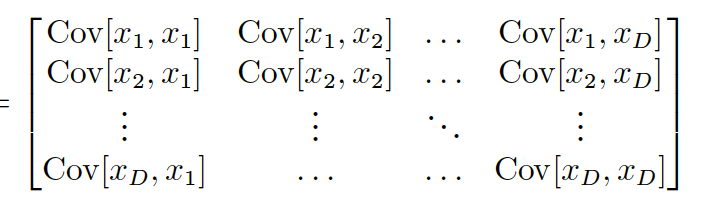
\includegraphics[width=0.6 \textwidth]{sections/images/prob1.png}
 
 It is symmetric and postive semidefinite. \\
 The \textit{correlation} statistics is the normalization of the covariance, where each rv $x$ is divided by its standard deviation $\sigma(x)$.

 \begin{definition}
     We define the \textit{correlation} between two random variables $X$ and $Y$ as
     $$ \text{Corr}(x, y) = \frac{\text{Cov}(x, y)}{\sigma(x)\sigma(y)} \ \ in [-1,1]$$
 \end{definition}

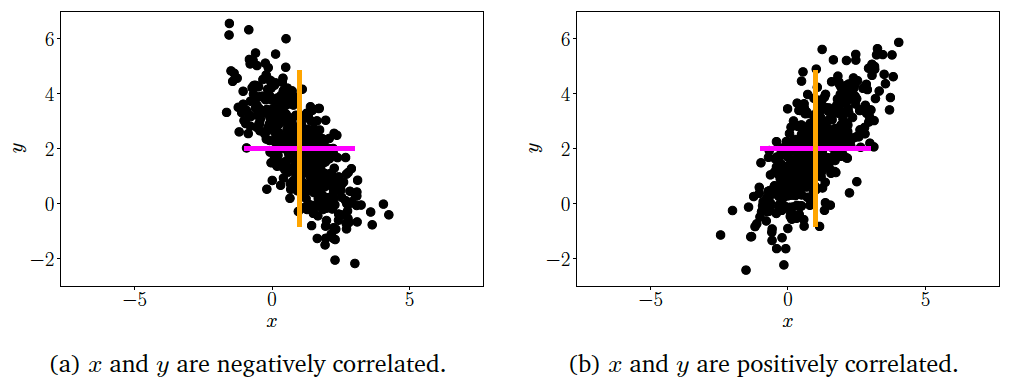
\includegraphics[width=0.6 \textwidth]{sections/images/prob2.png}

%If $X \in \set{R}^m,\ X = (X_1, X_2, \hdots, X_m)$ and $Y \in \set{R}^n,\ Y = (Y_1, Y_2, \hdots, Y_n)$ we have that $\text{Cov}(X, Y)$ and $\text{Corr}(X, Y)$ are matrices of size $m \times n$ such that
%$$ (\text{Cov}(X, Y))_{ij} = \text{Cov}(X_i, Y_j) $$
%$$ (\text{Corr}(X, Y))_{ij} = \text{Corr}(X_i, Y_j) $$



The previous statistics are also called \textit{population mean and (co)variance} since they are computed on the true population distribution.

 \subsection{Inferential statistics}
 Inferential statistics tries to deduce underlying properties of the distribution of a population from which a sample is observed. In ML we deal with empirical data and we aim to learn from them information on the true distribution they belong. 
 
 %The set of assumptions is called \textit{statistical model} and the assumed probability distribution is usually parametrized. These parameters are then estimated to fit the observed data as well as possible.

We have a finite dataset of $N$ samples and we use them to compute a statistic such as the mean or variance. In this case they are called \textit{empirical mean (covariance} or \textit{sample mean (covariance)}.

\begin{definition}
Suppose we have identical distributed univariate rv $X_1, \ldots X_n$ with corresponding realizations $x_1, \ldots x_n$. The empirical mean is defined as:
$$\bar x=\sum_{i=1}^N x_i $$
The empirical covariance is defined as:
$$\Sigma=\frac{1}{N} \sum_{i=1}^N (x_i-\bar x)^2$$
\end{definition}
In the case of multivariate rv $X_1, \ldots X_N$, $X_i \in \mathbb{R}^D$, the mean is a D vector of mean and the covariance is a $D \times D$ matrix 
$$\Sigma=\frac{1}{N} \sum_{i=1}^N (\xx_i-\bar \xx) (\xx_i-\bar \xx)T$$


\begin{definition}
$X$ and $Y$ rv are independent if $$p(\xx,\yy)=p(\xx)p(\yy)$$
\end{definition}

Hence:
\begin{itemize}
    \item $p(\yy|\xx)=p(\yy)$
    \item $p(\xx|\yy)=p(\xx)$
    \item $\mathbb{V}_{XY}{[\xx+\yy]}=\mathbb{V}_X[\xx](\xx)+\mathbb{V}_Y[\xx](\yy)$
    \item $\text{Cov}_{XY}[\xx,\yy]=0$
\end{itemize}

It can happen that $\text{Cov}_{XY}[\xx,\yy]=0$ but $X$,$Y$ are not statistically independent. (Ex. 6.5 MML)

If swe have more than twop rv, independent refers to mutually independent ($X_i, X_j, \ i\neq j$).

\subsection{Gaussian distribution}

Certainly, the most common distribution is the gaussian distribution (a continuous distribution) in different application areas (also ML).
In the case of univariate rv, the pdf of the gaussian distribution is:
$$p(x|\mu, \sigma^2)=\frac{1}{\sqrt{2 \pi \sigma^2}} exp \left(-\frac{(x-\mu)^2)}{2\sigma^2}\right)$$
We write: $p(\xx)={N} (\xx|\vec{\mu},\vec{\Sigma})$

Multivariate gaussian distribution:
$$p(\xx|\vec{\mu},\vec{\Sigma})=(2\pi)^{-\frac{D}{2}}|\vec{\Sigma}|^{-\frac{1}{2}}exp(-\frac{1}{2}(\xx-\vec{\mu})^T \vec{\Sigma}^{-1}(\xx-\vec{\mu}))$$

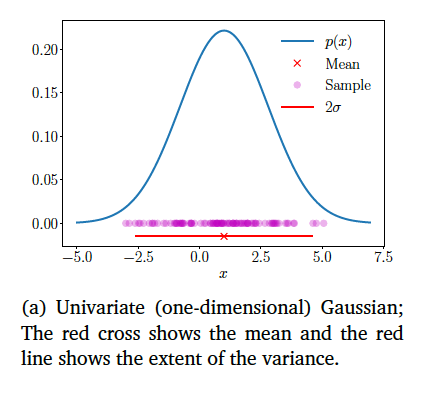
\includegraphics[width=0.6 \textwidth]{sections/images/prob3.png}

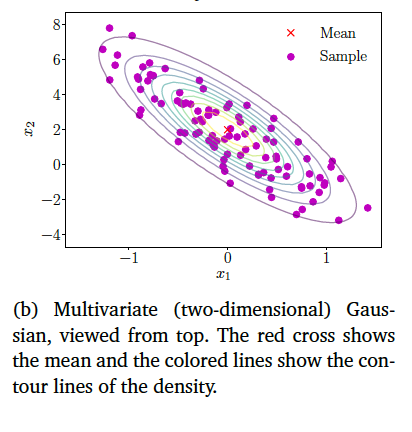
\includegraphics[width=0.6 \textwidth]{sections/images/prob4.png}

In the case $\mu=0, \sigma=1$ we have the normal distribution.

The conditional and marginal distributions of gaussian has a closed form.
If we consider the probability:

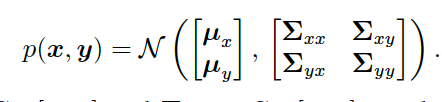
\includegraphics[width=0.6 \textwidth]{sections/images/prob5.png}

with $\Sigma_{xx}=\text{Cov}[x,x]$, $\Sigma_{yy}=\text{Cov}[y,y]$ the marginal covariance matrices of $\xx$ and $\yy$, $\Sigma_{xy}=\text{Cov}[x,y]$ the cross covariance matrix between $\xx$ and $\yy$. Then:

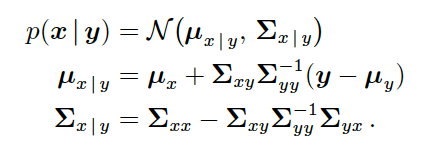
\includegraphics[width=0.6 \textwidth]{sections/images/prob6.png}

The marginal distribution:

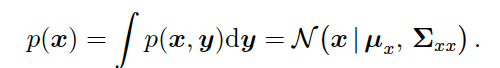
\includegraphics[width=0.6 \textwidth]{sections/images/prob7.png}

Example 6.6 MML.
